\documentclass[a4paper,10pt,oneside]{article}
\usepackage{graphicx}
\usepackage{color}
\usepackage{url}
\usepackage{subfigure}
\usepackage[utf8]{inputenc}
\usepackage[T1]{fontenc}
\usepackage{tgpagella}
%\usepackage[scale=0.9]{tgcursor}
%\usepackage[scale=0.9]{tgheros}

\newcommand{\myscale}{0.74}
\newcommand{\vect}[1]{\boldsymbol{#1}}
\newcommand{\code}[1]{\texttt{#1}}
\newcommand{\jmodule}[1]{\texttt{\textit{#1}}}

\setlength{\hoffset}{-1in} %left margin will be 0, as hoffset is by default 1inch
\setlength{\voffset}{-1in} %analogous voffset
\setlength{\oddsidemargin}{1.5cm}
\setlength{\evensidemargin}{1.5cm}
\setlength{\topmargin}{1.5cm}
\setlength{\textheight}{24cm}
\setlength{\textwidth}{18cm}

\def\mftitle{jInfer BasicRuleDisplayer Module Description}
\def\mfauthor{Michal Klempa, Mário Mikula, Robert Smetana, Michal Švirec, Matej Vitásek}
\def\mfadvisor{RNDr. Irena Mlýnková, Ph.D., Martin Nečaský, Ph.D.}
\def\mfplacedate{Praha, 2011}
\title{\bf\mftitle}
\author{\mfauthor \\ Advisors: \mfadvisor}
\date{\mfplacedate}

\ifx\pdfoutput\undefined\relax\else\pdfinfo{ /Title (\mftitle) /Author (\mfauthor) /Creator (PDFLaTeX) } \fi

\begin{document}
\maketitle
\noindent Target audience: developers willing to extend jInfer, looking for ways to visualize grammars.

\noindent \begin{tabular}{|l|l|} \hline
Responsible developer: & Matej Vitásek \\ \hline
Required tokens:       & none \\ \hline
Provided tokens:       & cz.cuni.mff.ksi.jinfer.base.interfaces.RuleDisplayer \\ \hline
Module dependencies:   & Base \\ \hline
Public packages:       & none \\ \hline
\end{tabular}

\section{Introduction}

This is fairly basic rule displayer draws rules as series of nested coloured rectangles. It does so by recursively descending down the regexp tree to draw the innermost nodes first, composing the outer nodes from them. User interface-wise, it creates a component with multiple panels: each one for a new grammar to display.

\section{Structure}

The main class implementing \code{RuleDisplayer} inference interface and simultaneously registered as its service provider is \code{BasicRuleDisplayer}. Main method of this class is \code{createDisplayer()}, which looks up the component, adds a new panel to it and renders the specified grammar in it.\\

\begin{figure}
	\centering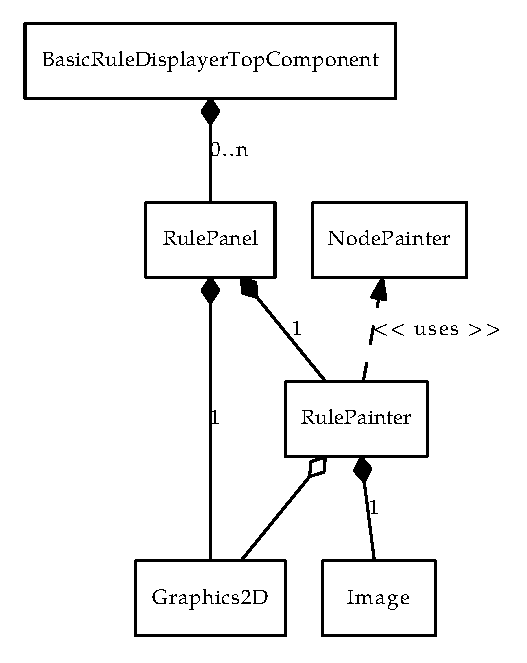
\includegraphics[scale=\myscale]{class-diagram}
	\caption{BasicRuleDisplayer class diagram} \label{figure-class-diagram}
\end{figure}

The diagram of classes involved in rule display is in figure \ref{figure-class-diagram}. The top component of the rule displayer has a few panels in it: each contains its own \code{RuleDisplayer} responsible for rendering specified grammar once into an internal \code{Image}, then keeping it and drawing it onto panel's \code{Canvas} each time repainting is needed.\\

Grammar is rendered in the \code{drawRules()} method by recursively rendering its rules and stacking their image representations into the image. Rule painting is handled in the \code{NodePainter} class, with most important method \code{drawNode()}. While the code itself is a nice recursion programming exercise, there is nothing of a special interest in it.\\

All graphics used by \jmodule{BasicRuleDisplayer} is contained in the \code{cz.cuni.mff.ksi.jinfer.basicruledisplayer.graphics} package.

\subsection{Settings}

All settings provided by \jmodule{BasicRuleDisplayer} are NetBeans-wide. The options panel along with all the logic is in the \code{cz.cuni.mff.ksi.jinfer.basicruledisplayer.options} package. Available options include setting the maximum number of panels concurrently displayed, rules drawn, as well as maximum nesting level. Everything beyond these limits will be rendered as an icon suggesting omitted information. Furthermore, colours of various nodes can be set here.

%\nocite{*}
\newpage
\bibliographystyle{alpha}
\bibliography{literature}

\end{document}
